\section{Stand der Technik}

Für die Bezahlungsmethoden werden hier zweiverschiedene Arten von Zahlungsverfahren analysiert und deren
Vorteile in Bezug auf Sicherheit und Härtungsmaßnahmen dargestellt: drahtlose Zahlung und Kartenzahlung.

\subsection{Drahtlose Verbindungen und Sicherheit bei Bezahlungen}

Viele digitale Zahlungen finden über WLAN statt, was ein großes Risiko darstellen kann \cite{refip:NYRS}, 
da WLAN-Verbindungen nicht so sicher sind wie Kabelverbindungen. Maßnahmen zu entwickeln, die sich an 
verschiedenen Systeme anpassen, kosten Zeit und Investitionen von Banken und Sicherheitsfirmen. 
Für jeden möglichen Angriffe sollte präventiv etwas getan werden, sodass die Integrität des Kunden 
geschützt bleibt. Die folgenden Schwachstellen bei digitaler Zahlung wurden von \cite{refip:NYRS}
zusammengefasst:

\begin{itemize}
    \item Erstellung von Dateien in dem Opfersystem mit umfangreichen Privilegien;
    \item Unzureichende Sicherheit bei der Validierung von Zertifikaten;
    \item Quellcode ist öffentlich zugänglich, sodass das Opfersystem von Reverse
    Engineering betroffen sein könnte
    \item Unsicherer Umgang mit Cookies-Einstellungen
\end{itemize}

\cite{refip:NYRS} schlägt einige Sicherheitsmechanismen vor, die die oben gennanten Schwachstellen bei 
kabelosen Verbindungen reduzieren können. Unter denen werden folgende hervorgehoben: 

\begin{itemize}
    \item Nutzung von modernen kryptographischen Standards für die Validierung von Zertifikaten;
    \item Erstellung von Loggdatei, sodass jeder Anormalität schnell überprüft werden kann;
    \item Zwei-Faktor-Authentifizierung;
    \item Digitale und zufällig geordnete Tastatur;
    \item Schwierigkeitsgrad bei der Erstellung von Passwörtern;
    \item Besserer Umgang mit der Verwaltung von Cookies;
    \item Registrierung von Geräten;
    \item Künstliche Intelligenz (KI) für die Detektion von abweichenden Verhalten;
    \item Ständige Kontrolle gegen Social Engineering.
\end{itemize}


Kredit- und EC-Karten sollen auch als Zahlungsmittel bei unserem Click and Buy Automat
akzeptiert werden. In Bezug auf diese Zahlungsmittel, wird die Sicherheit im folgenden untersucht.


\subsection{Anwendung von Smartcards und sicheres Bezahlen}
Der Begriff Smartcards bezeichnet eine Plastikkarte mit einem eingebauten Chip, der ein eigenes 
Betriebssystem, einen Mikroprozessor und minimale Funktionalitäten besitzt \ref{fig:eigenes_Bild}. 

\vfill
\begin{figure}[H]
   \centering{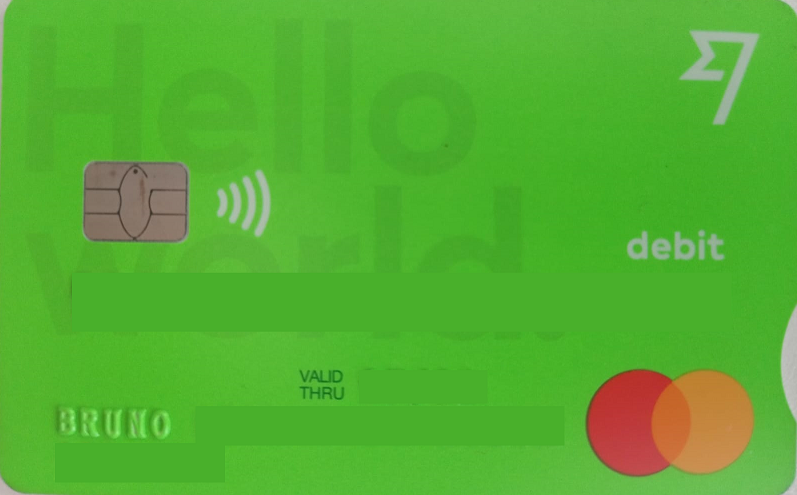
\includegraphics[width=10cm]{Bilder/eigenes_Bild_Karte.png}}
   \caption{Eine Smartcard und deren eingebetete Mikrochip\\(eigene Quelle)}
   \label{fig:eigenes_Bild}
\end{figure}
\vfill

Sie wurde vor mehr als 40 Jahren erfunden und ihr Ziel ist die Sicherheit von Kartenzahlung und allgemeine
Authentifizierungsverfahren zu erhöhen \cite{refip:JFSB}. Sie unterscheiden sich von traditionelen 
Magnetstreifenkarten, weil sie verschiedene Authentifizierungsmethoden ermöglichen auch ohne direkte 
Verbindung zur Bank \cite{refbook:ATMS}. Im folgenden wird der Authentifizierungsprozess einer Smartcard 
\ref{fig:refbook_ATMS} dargestellt. 


\vfill
%htb
\begin{figure}[H]
    \centering{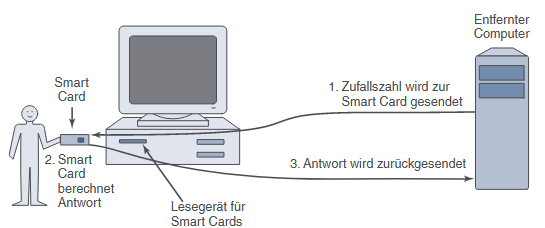
\includegraphics[width=10cm]{Bilder/refbook_ATMS.png}}
   \caption{Authentifizierungsprozess von Smartcards\\(Tanenbaum, 2009, S.755)}
   \label{fig:refbook_ATMS}
\end{figure}
\vfill

Die meisten Angriffe bei Smartcards geschehen laut \cite{refmas:ASSS} auf Hardwareebene.
Er beschreibt folgende Techniken für Angriffe:

\begin{itemize}
    \item Protokollanalyse: schwache Konzipierung oder mangelnde Verschlüsselung ermöglichen den Zugang 
    zu dem Klartext; 
    \item Relay: Konzentriert auf kontaktlose Smartcards, um den Inhalt umzuleiten;
    \item Seitenkanal-Attacken: zielt nicht direkt den Inhalt des Kommunikation, sondern versucht sie
    irgendwie zu stören;
    \item Hardware Reverse Engineering: Verständnis über die Algorithmen oder Extrahieren des Schlüssels.
\end{itemize}


Die Schutzmaßnahmen können laut \cite{refmas:ASSS} in drei Gruppen aufgeteilt werden: physikalisch,
logisch und organisatorisch. Auf der physikalischen Ebene soll die Hardware "robust" aufgebaut werden,
um Angriffe schwieriger zu gestalten. Diese Konstruktion soll komplex mit zusätzlichen Elementen erstellt
werden. 



================== --> das verstehe ich auch nicht so ganz 
Auf der logischen Ebenen sollen moderne und starke Verschlüsselungsverfahren
eingesetzt werden, die gegen Sicherheitslücken überprüft wurde. Die Bearbeitungszeit spielt hier
eine wesentliche Rolle gegen Angriffe, die auf Seitkanäle basiert sind. 
==================


Letztendlich sollen Smartcards in der Lage sein, Angriffe schnell zu detektieren und zu verhindern.
Zu dieser Ebene gehört auch das Sperren der Karte, falls die Karte unautorisiert genutzt wurde, 
die Überprüfung von Logdateien, um Klone zu identifizieren und die Verwendung von Zwei-Faktor-
Authentisierung.
